\documentclass[xcolor=dvipsnames,t,aspectratio=169]{beamer}

\usecolortheme{rose}
\usecolortheme{dolphin}
\usetheme{Boadilla}

\input{../../templates/slides/imports}
\input{../../templates/slides/settings}
\input{../../templates/slides/commands}

\titlegraphic{
    \includegraphics[scale = 0.5]{../../templates/slides/logo}
}

\logo{
\begin{tikzpicture}[overlay,remember picture]
\node[xshift=-.75cm, yshift=-1cm] at (current page.30){
    \includegraphics[width=0.1\textwidth]{../../templates/slides/logo}};
\end{tikzpicture}
}
\usetikzlibrary{positioning}

\newcommand{\highlight}[1]{{\color{nes_dark_orange} #1}}

\title{Git, Github e Ambientes de Desenvolvimento}

\author{Eduardo Adame}

\date{{\color{nes_dark_purple}\textbf{Ciência de Dados}\\[0.5em] 11 de março de 2026 }}

\begin{document}

\frame[plain]{\titlepage}
\setcounter{framenumber}{0}

\section{Controle de Versão}

\begin{frame}[c]{Por que controle de versão?}

Problemas comuns em projetos:

\begin{itemize}

\item Arquivos chamados:

\begin{itemize}
\item analysis\_final.py
\item analysis\_final\_v2.py
\item analysis\_final\_definitivo.py
\end{itemize}

\item Mudanças irreversíveis
\item Colaboração difícil
\item Código quebrando sem saber quando
\end{itemize}

\begin{display}[Objetivo do Git]

Rastrear mudanças em arquivos ao longo do tempo.

\end{display}

\end{frame}


\section{Como Git funciona}

\begin{frame}[c]{Snapshots, não diffs}

Git armazena o estado do projeto como \highlight{snapshots}.

\begin{center}

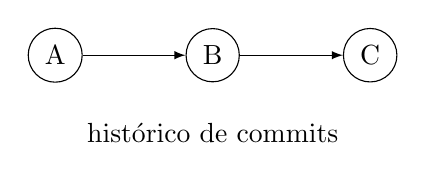
\begin{tikzpicture}[node distance=2cm]

\node (a) [circle,draw] {A};
\node (b) [circle,draw,right of=a] {B};
\node (c) [circle,draw,right of=b] {C};

\draw[-latex] (a) -- (b);
\draw[-latex] (b) -- (c);

\node[below=0.4cm of b] {histórico de commits};

\end{tikzpicture}

\end{center}

Cada commit contém:

\begin{itemize}

\item snapshot dos arquivos
\item autor
\item mensagem
\item hash SHA
\end{itemize}

\end{frame}


\begin{frame}[c]{Estrutura interna}

Componentes principais:

\begin{itemize}

\item Working Directory
\item Staging Area
\item Repository
\end{itemize}

\begin{center}


\begin{tikzpicture}[node distance=5cm]

\node (w) [rectangle,draw] {Working directory};

\node (s) [rectangle,draw,right of=w] {Staging};

\node (r) [rectangle,draw,right of=s] {Repository};

\draw[-latex] (w) -- node[above]{git add} (s);
\draw[-latex] (s) -- node[above]{git commit} (r);

\end{tikzpicture}

\end{center}

\end{frame}


\section{Comandos essenciais}

\begin{frame}[c, fragile]{Criando um repositório}

\begin{code}[Inicializando repositório]{bash}
git init
git add file.py
git commit -m "first commit"
\end{code}

\end{frame}


\begin{frame}[c, fragile]{Trabalhando com remotes}

\begin{code}[Clonar repositório]{bash}
git clone git@github.com:adamesalles/ciencia-de-dados.git
\end{code}

\begin{code}[Enviar alterações]{bash}
git push origin main
\end{code}

\begin{code}[Atualizar repositório]{bash}
git pull
\end{code}

\end{frame}


\section{Branches}

\begin{frame}[c]{Branching}

Branches permitem desenvolver funcionalidades isoladamente.

\begin{center}

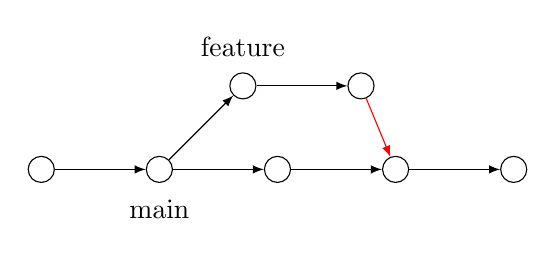
\begin{tikzpicture}[node distance=1.5cm]

\node (a) [circle,draw] {};
\node (b) [circle,draw,right of=a] {};
\node (c) [circle,draw,right of=b] {};
\node (f) [circle,draw,right of=c] {};
\node (g) [circle,draw,right of=f] {};

\node (d) [circle,draw,above right of=b] {};
\node (e) [circle,draw,right of=d] {};

\draw[-latex] (a) -- (b);
\draw[-latex] (b) -- (c);
\draw[-latex] (c) -- (f);
\draw[-latex] (f) -- (g);

\draw[-latex] (b) -- (d);
\draw[-latex] (d) -- (e);
\draw[-latex, red] (e) -- (f);

\node[below of=b, yshift=1cm] {main};
\node[above of=d, yshift=-1cm] {feature};

\end{tikzpicture}

\end{center}

\begin{figure}[h]
    \centering
    \includegraphics[width=0.4\linewidth]{gittree.png}
\end{figure}

\end{frame}


\begin{frame}[c, fragile]{Criando branch}

\begin{code}[Branch]{bash}
git branch feature
git checkout feature

# ou

git checkout -b feature
\end{code}

\end{frame}

\section{Merge}

\begin{frame}[c]{Tipos de merge}

Tipos comuns:

\begin{itemize}

\item Fast-forward
\item Merge commit
\item Rebase
\end{itemize}

Fast-forward ocorre quando não há divergência no histórico. 

\end{frame}



\begin{frame}[c, fragile]{Amend}

Corrigir último commit:

\begin{code}[Amend]{bash}
git commit --amend
git push --force-with-lease # cuidado!!
\end{code}

Usos comuns:

\begin{itemize}

\item corrigir mensagem
\item adicionar arquivo esquecido
\end{itemize}

\end{frame}

\begin{frame}[c, fragile]{Issues e Pull Requests}

\textbf{Issues} são usadas para organizar tarefas, bugs e novas funcionalidades.

\begin{itemize}
\item Cada issue representa um \highlight{problema ou tarefa}
\item Possui número único: \texttt{\#12}
\item Pode ter responsáveis, labels e discussões
\end{itemize}

\textbf{Pull Requests (PR)} são propostas de mudança no código.

\begin{itemize}
\item Um branch é enviado para revisão
\item Outros desenvolvedores podem comentar e revisar
\item Após aprovação, o código é integrado ao branch principal
\end{itemize}

\end{frame}

\begin{frame}[c, fragile]{Issues e Pull Requests}


Podemos mencionar issues usando \texttt{\#numero}.

\begin{code}[Referência em commit]{bash}
git commit -m "implementa leitura de palavras (#12)"
\end{code}


Algumas palavras-chave fecham a issue quando o commit/PR é integrado ao branch principal:

\begin{code}[Fechando issue automaticamente]{bash}
git commit -m "implementa lógica do jogo. closes #12"
\end{code}

Palavras aceitas: \texttt{close, closes, closed, fix, fixes, fixed, resolve, resolves, resolved}.

\end{frame}


\section{Git vs GitHub}

\begin{frame}[c]{Git vs GitHub}

\begin{columns}

\begin{column}{0.5\textwidth}

Git:

\begin{itemize}

\item ferramenta
\item controle de versão
\item local

\end{itemize}

\begin{figure}
\centering
\includegraphics[height=.3\textheight]{images/gitlogo.png}
\end{figure}

\end{column}

\begin{column}{0.5\textwidth}

GitHub / GitLab:

\begin{itemize}

\item hospedagem de repositórios
\item colaboração
\item CI/CD
\end{itemize}

\begin{figure}
\centering
\includegraphics[height=.3\textheight]{images/github-logo.png}
\end{figure}

\end{column}

\end{columns}

\end{frame}


\section{Ambientes}

\begin{frame}[c]{Script vs Notebook}

\begin{columns}

\begin{column}{0.5\textwidth}

Script

\begin{itemize}

\item executável
\item reprodutível
\item melhor para produção
\item múltiplos arquivos
\item funciona bem com git
\end{itemize}

\begin{figure}
\centering
\includegraphics[height=.3\textheight]{images/Python-logo-notext.svg.png}
\end{figure}

\end{column}

\begin{column}{0.5\textwidth}

Notebook

\begin{itemize}

\item exploratório
\item visual
\item documentação interativa
\item melhor para protótipos
\item não funciona bem com git
\end{itemize}

\begin{figure}
\centering
\includegraphics[height=.3\textheight]{images/jupyter-logo.png}
\end{figure}

\end{column}

\end{columns}

\end{frame}


\begin{frame}[c]{IDEs}

\begin{figure}[ht]
\centering
\begin{subfigure}{0.2\textwidth}
\centering
\includegraphics[width=\textwidth]{images/vscode-logo.png}
\caption*{Visual Studio Code}
\end{subfigure}
\hfill
\begin{subfigure}{0.2\textwidth}
\centering
\includegraphics[width=\textwidth]{images/nvim-icon.png}
\caption*{Neovim}
\end{subfigure}
\hfill
\begin{subfigure}{0.2\textwidth}
\centering
\includegraphics[width=\textwidth]{images/rstudio-logo.png}
\caption*{R Studio}
\end{subfigure}

\begin{subfigure}{0.2\textwidth}
\centering
\includegraphics[width=\textwidth]{images/windsurf.png}
\caption*{Windsurf}
\end{subfigure}
\hfill
\begin{subfigure}{0.2\textwidth}
\centering
\includegraphics[width=\textwidth]{images/pycharm.png}
\caption*{PyCharm}
\end{subfigure}
\hfill
\begin{subfigure}{0.2\textwidth}
\centering
\includegraphics[width=\textwidth]{images/positron-logo.png}
\caption*{Positron}
\end{subfigure}
\end{figure}

\end{frame}


\section{Gerenciamento de pacotes}

\begin{frame}[c, fragile]{Gerenciadores}

    \begin{columns}

        \begin{column}{0.3\textwidth}
            \begin{itemize}

            \item pip
            \item conda
            \item pipenv
            \item poetry
            \item uv
            \end{itemize}
        \end{column}

        \begin{column}{0.7\textwidth}
            \begin{code}[Criar projeto]{bash}
            uv init project
            \end{code}

            \begin{code}[Adicionar dependência]{bash}
            uv add pandas
            \end{code}

            Arquivo central:

            \begin{code}[Config]{toml}
            {nvim, code} pyproject.toml
            \end{code}
        \end{column}
    \end{columns}


\end{frame}



\begin{frame}[c, c, noframenumbering, plain]
    \frametitle{~}
        \vfill
        \begin{center}
            {\Huge Obrigado!}\vspace{1.5em}\\
            {\Large \highlight{Alguma dúvida?}}\\
        \end{center}
        \vfill
        \begin{center}
            {\small Agora vamos para os exercícios!}
        \end{center}
\end{frame}

\end{document}